\documentclass{report}

\usepackage[T2A]{fontenc}
\usepackage[utf8]{inputenc}
\usepackage[russian]{babel}

\usepackage{misccorr}
\usepackage{indentfirst}

\usepackage{setspace}
\onehalfspace

\usepackage{graphicx}

\usepackage{listings}
\lstset{captionpos=b}

\usepackage{amsmath}

\begin{document}

\tableofcontents

\chapter*{Введение}
\addcontentsline{toc}{chapter}{Введение}

В различных областях науки и техники довольно часто встречается
задача определения схожести строк. Например, набранные вручную
документы могут содержать опечатки, требующие исправления. Другой
пример: полученные с помощью телекоммуникации данные могут
содержать различные искажения из-за помех на линии. Для решения
подобных задач применяют разнообразные метрики схожести строк,
одними из которых являются расстояния Левенштейна и
Дамерау-Левенштейна.

\chapter{Аналитическая часть}

Пусть $\textbf{s}$ и $\textbf{t}$ -- строки над некоторым алфавитом
$V$, причём

$$
|\textbf{s}| = m, |\textbf{t}| = n.
$$

Расстояние Левенштейна определяется как минимальное количество
редакционных операций, необходимых для превращения одной строки в
другую.

Под редакционными операциями здесь понимают следующие действия над
строками:

\begin{itemize}
    \item вставка одного символа;
    \item удаление одного символа;
    \item замена одного символа на другой.
\end{itemize}

Расстояние Левенштейна
$\Delta_{\textup{Л}}(\textbf{s}, \textbf{t})$ между строками
$\textbf{s}$ и $\textbf{t}$ может быть вычислено как
$d_{\textup{Л}}(m, n)$, где

\begin{equation} \label{eq:vl}
    d_{\textup{Л}}(i, j) =
    \begin{cases}
        0, i = 0, j = 0;
        \\
        j, i = 0, j > 0;
        \\
        \min
        \begin{cases}
            d_{\textup{Л}}(i, j - 1) + 1,
            \\
            d_{\textup{Л}}(i - 1, j) + 1,
            \\
            d_{\textup{Л}}(i - 1, j - 1) + \delta(i, j).
        \end{cases}
    \end{cases}
\end{equation}

Здесь и далее

$$
\delta(i, j) =
\begin{cases}
    \textup{если $\textbf{s}_i = \textbf{t}_j$, то }
    0;
    \\
    \textup{иначе }
    1.
\end{cases}
$$

В свою очередь, расстояние Дамерау-Левенштейна учитывает то
обстоятельство, что наиболее частой ошибкой при наборе человеком
текстов на клавиатуре является перестановка (транспозиция) двух
символов. Таким образом, под редакционными операциями здесь
понимают чуть более широкий набор действий над строками:

\begin{itemize}
    \item вставка одного символа;
    \item удаление одного символа;
    \item замена одного символа на другой;
    \item перестановка двух символов.
\end{itemize}

Расстояние Дамерау-Левенштейна
$\Delta_{\textup{ДЛ}}(\textbf{s}, \textbf{t})$ между строками
$\textbf{s}$ и $\textbf{t}$ может быть вычислено как
$d_{\textup{ДЛ}}(m, n)$, где

\begin{equation} \label{eq:dl}
    d_{\textup{ДЛ}}(i, j) =
    \begin{cases}
        0, i = 0, j = 0;
        \\
        j, i = 0, j > 0;
        \\
        \textup{если $\gamma(i, j)$, то}
        \min
        \begin{cases}
            d_{\textup{ДЛ}}(i, j - 1) + 1,
            \\
            d_{\textup{ДЛ}}(i - 1, j) + 1,
            \\
            d_{\textup{ДЛ}}(i - 1, j - 1) + \delta(i, j),
            \\
            d_{\textup{ДЛ}}(i - 2, j - 2) + 2;
        \end{cases}
        \\
        \textup{иначе}
        \min
        \begin{cases}
            d_{\textup{Л}}(i, j - 1) + 1,
            \\
            d_{\textup{Л}}(i - 1, j) + 1,
            \\
            d_{\textup{Л}}(i - 1, j - 1) + \delta(i, j).
        \end{cases}
    \end{cases}
\end{equation}

Здесь

$$
\gamma(i, j) =
\begin{cases}
    i, j > 1;
    \\
    \textbf{s}_i = \textbf{t}_{j - 1};
    \\
    \textbf{s}_{i - 1} = \textbf{t}_j.
\end{cases}
$$

На практике расстояния Левенштейна и Дамерау-Левенштейна могут
быть вычислены с помощью различных алгоритмов.

Цель данной работы -- изучить метод динамического программирования
на примере реализации алгоритмов поиска расстояний Левенштейна и
Дамерау-Левенштейна.

Для этого необходимо решить следующие задачи:

\begin{enumerate}
    \item изучить расстояния Левенштейна и Дамерау-Левенштейна;
    \item разработать алгоритмы поиска изученных расстояний;
    \item реализовать разработанные алгоритмы;
    \item выполнить замеры процессорного времени работы реализаций;
    \item оценить объём требуемой для работы реализаций памяти;
    \item выполнить сравнительный анализ разработанных алгоритмов.
\end{enumerate}

\chapter{Конструкторская часть}

Были разработаны следующие алгоритмы:

\begin{itemize}
    \item поиска расстояния Левенштейна:
    \begin{itemize}
        \item нерекурсивный;
    \end{itemize}
    \item поиска расстояния Дамерау-Левенштейна:
    \begin{itemize}
        \item нерекурсивный;
        \item простой рекурсивный;
        \item рекурсивный с кэшем.
    \end{itemize}
\end{itemize}

\section{Поиск расстояния Левенштейна}

\subsection{Нерекурсивный алгоритм} \label{design-vl-iterative}

Заполним целочисленную матрицу $D$ размером $(m + 1)(n + 1)$ таким
образом, что $d_{ij}$ -- расстояние Левенштейна между срезами
$\textbf{s}_1^{i - 1}$ и $\textbf{t}_1^{j - 1}$, где

$$
\textbf{x}_m^n = \textbf{x}_m \textbf{x}_{m + 1} ... \textbf{x}_n.
$$

Это можно сделать с помощью двух вложенных циклов. В таком случае,
$\Delta_{\textup{Л}} = d_{ij}$ при $i = m + 1, j = n + 1$. Схема
этого алгоритма приведена на рисунке \ref{fig:vl-iterative}.

\begin{figure}
    \centering
    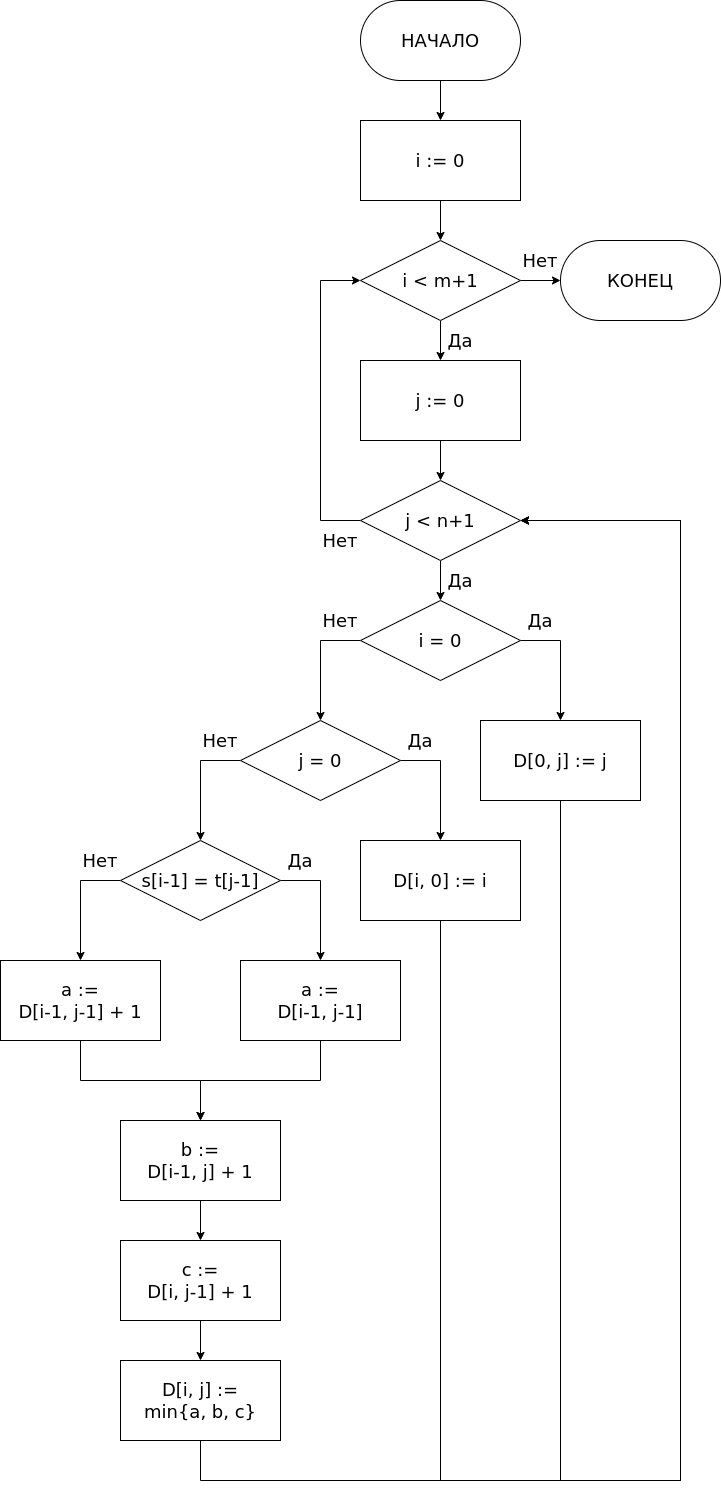
\includegraphics[height=0.8\textheight]{alg-vl-iterative.png}
    \caption{Схема нерекурсивного алгоритма поиска
        $\Delta_{\textup{Л}}$}
    \label{fig:vl-iterative}
\end{figure}

\section{Поиск расстояния Дамерау-Левенштейна}

\subsection{Нерекурсивный алгоритм}

Аналогично алгоритму из подраздела \ref{design-vl-iterative} был
разработан нерекурсивный алгоритм поиска расстояния
Дамерау-Левенштейна.

Cхема этого алгоритма представлена на рисунке
\ref{fig:dl-iterative}.

\begin{figure}
    \centering
    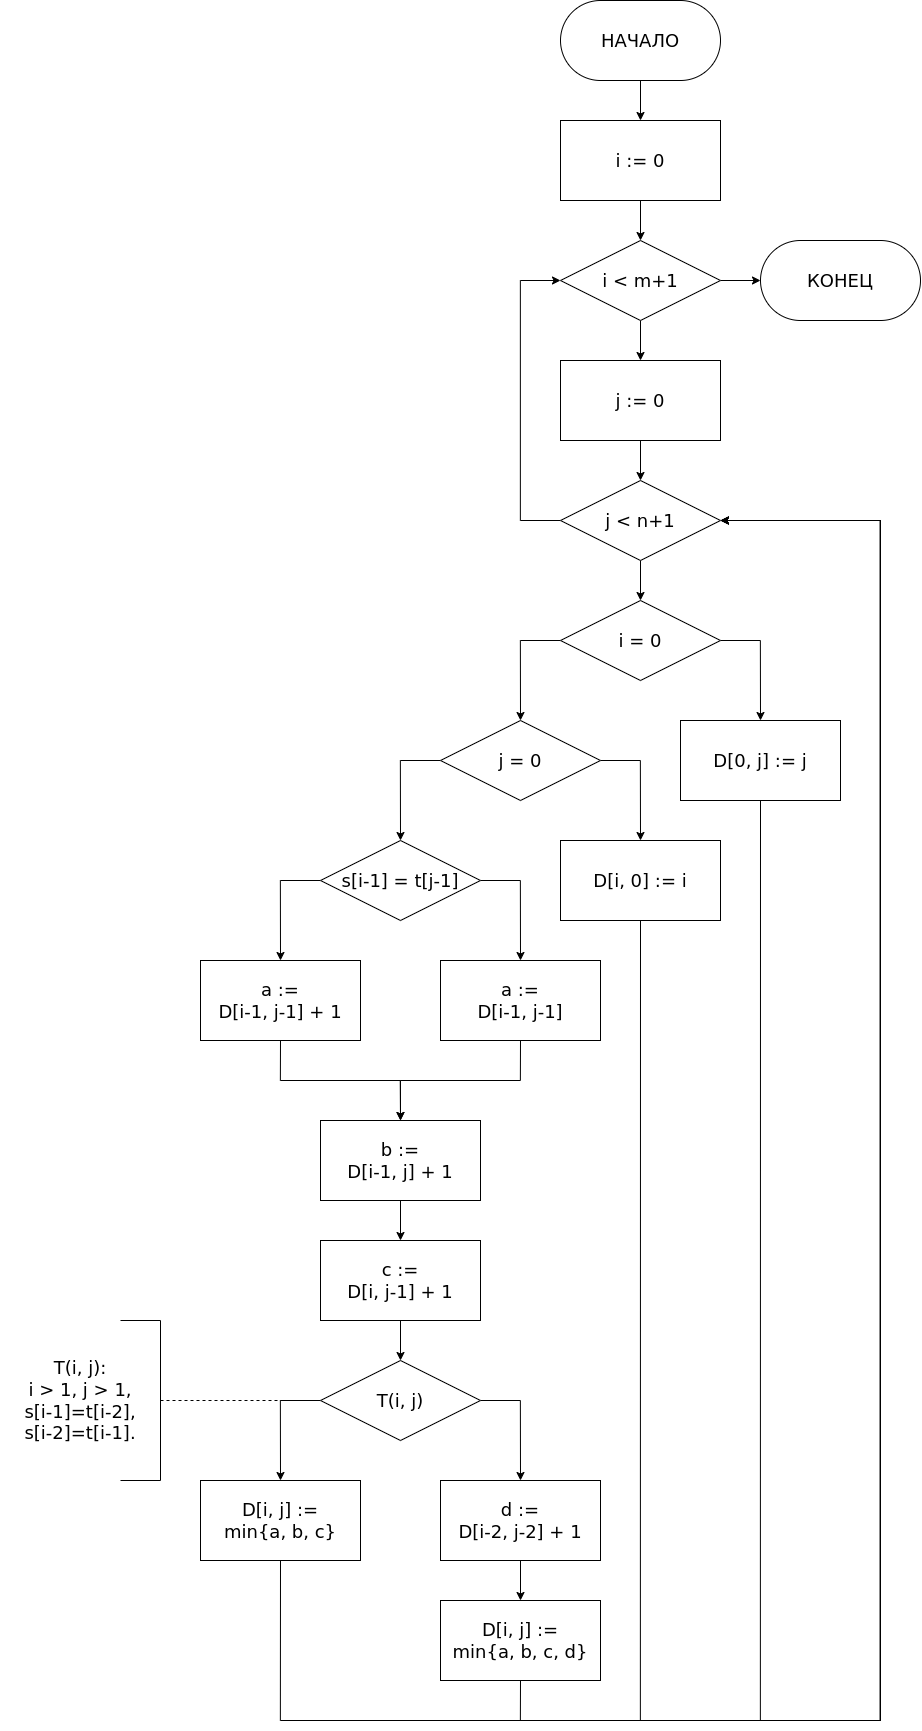
\includegraphics[height=0.8\textheight]{alg-dl-iterative.png}
    \caption{Схема нерекурсивного алгоритма поиска
        $\Delta_{\textup{ДЛ}}$}
    \label{fig:dl-iterative}
\end{figure}

\subsection{Простой рекурсивный алгоритм}

Расстояние Дамерау-Левенштейна также может быть вычислено
непосредственно по формуле \ref{eq:dl} с помощью рекурсивной
функции.

Схема этого алгоритма представлена на рисунке
\ref{fig:dl-recursive}.

\begin{figure}
    \centering
    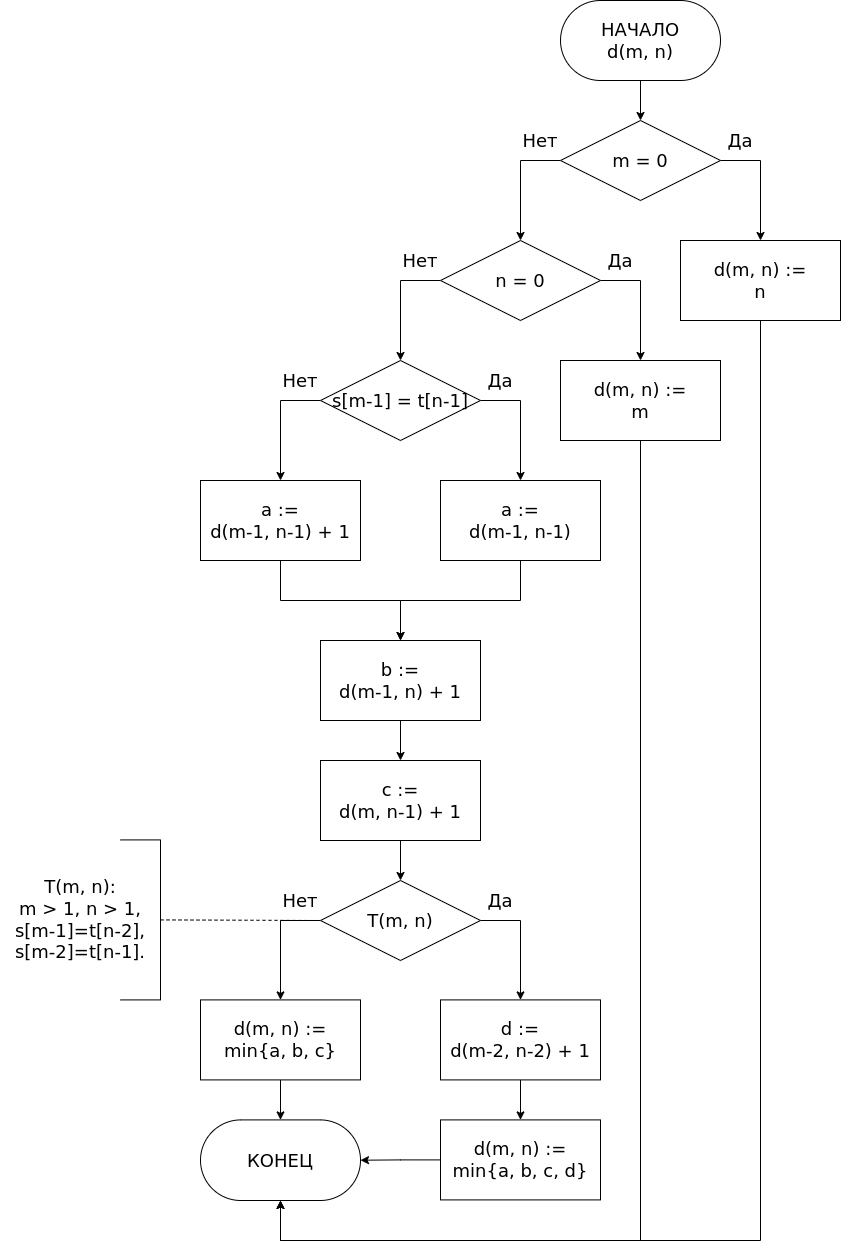
\includegraphics[height=0.8\textheight]{alg-dl-recursive.png}
    \caption{Схема простого рекурсивного алгоритма поиска
        $\Delta_{\textup{ДЛ}}$}
    \label{fig:dl-recursive}
\end{figure}

\subsection{Рекурсивный алгоритм с кэшем}

Главная проблема простого рекурсивного алгоритма поиска расстояния
Дамерау-Левенштейна в том, что многие значения выражения
\ref{eq:dl} вычисляются повторно. Очевидным решением является
введение кэша в виде матрицы $C$, подобной рассмотренной в
подразделе \ref{design-vl-iterative} матрице $D$, но допускающей
<<отсутствие>> значения одного или нескольких элементов.

Схема этого алгоритма представлена на рисунке
\ref{fig:dl-memoizing}.

\begin{figure}
    \centering
    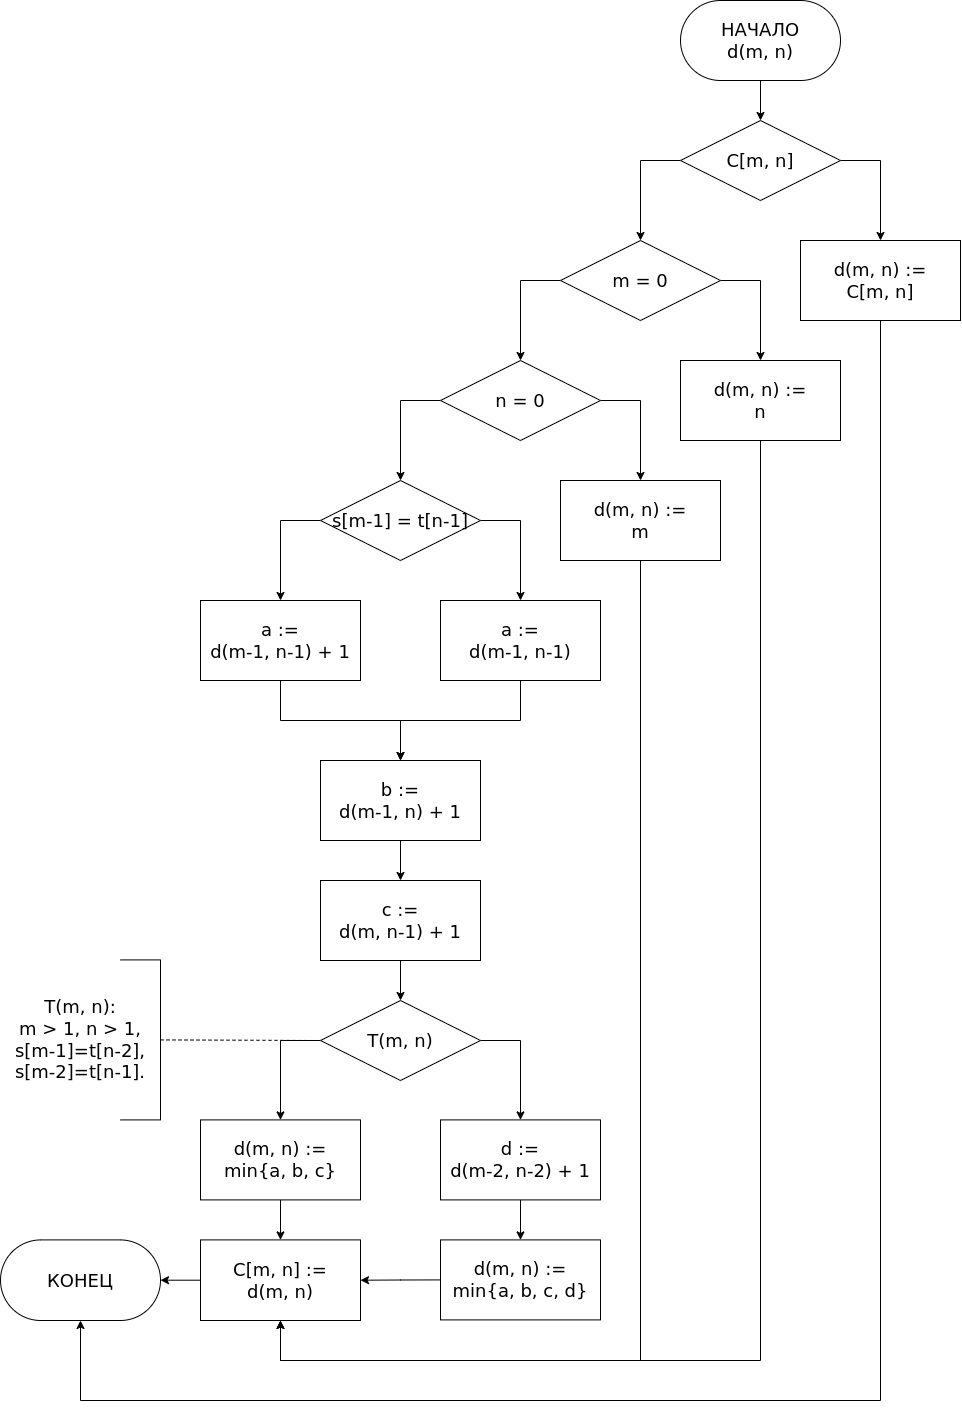
\includegraphics[height=0.8\textheight]{alg-dl-memoizing.png}
    \caption{Схема рекурсивного алгоритма с кэшем поиска
        $\Delta_{\textup{ДЛ}}$}
    \label{fig:dl-memoizing}
\end{figure}

\chapter{Технологическая часть}

\section{Средства разработки}

Для реализации разработанных алгоритмов был выбран язык
программирования Rust, поскольку он предоставляет высокую степень
контроля за ошибками во время компиляции.

Также для разработки, тестирования и отладки программ был
использован инструмент Cargo, поскольку он позволяет
автоматизировать значительную часть работы.

Для замера процессорного времени был выбран крейт
\texttt{cpu-time}, поскольку он предоставляет простой и
идиоматичный интерфейс.

\section{Реализации алгоритмов}

\subsection{Поиск расстояния Левенштейна}

В ходе работы был реализован нерекурсивный алгоритм поиска
расстояния Левенштейна на Rust.

\begin{lstlisting}[caption=Реализация нерекурсивного алгоритма
    поиска $\Delta_{\textup{Л}}$]
fn distance(s: &str, t: &str) -> usize {
    let (m, n) = (s.len(), t.len());

    // A matrix of Levenshtein distances
    let mut matrix = Matrix::new(0, m + 1, n + 1);

    for i in 0..m + 1 {
        for j in 0..n + 1 {
            if i == 0 {
                matrix.set(0, j, j);
                continue;
            }

            if j == 0 {
                matrix.set(i, 0, i);
                continue;
            }

            // The current characters
            let c = s.chars().nth(i - 1).unwrap();
            let d = t.chars().nth(j - 1).unwrap();

            let mut cases = vec![
                matrix.get(i - 1, j - 1)
                    + if c == d { 0 } else { 1 }
            ];

            cases.push(matrix.get(i - 1, j) + 1);
            cases.push(matrix.get(i, j - 1) + 1);

            matrix.set(i, j,
                *cases.iter().min().unwrap()
            );
        }
    }

    *matrix.get(m, n)
}
\end{lstlisting}

\subsection{Поиск расстояния Дамерау-Левенштейна}

В ходе работы были реализованы три алгоритма поиска расстояния
Дамерау-Левенштейна на Rust: нерекурсивный, простой рекурсивный и
рекурсивный с кэшем.

\begin{lstlisting}[caption=Реализация нерекурсивного алгоритма
    поиска $\Delta_{\textup{ДЛ}}$]
fn distance(s: &str, t: &str) -> usize {
    let (m, n) = (s.len(), t.len());

    // A matrix of Damerau-Levenshtein distances
    let mut matrix = Matrix::new(0, m + 1, n + 1);

    for i in 0..m + 1 {
        for j in 0..n + 1 {
            if i == 0 {
                matrix.set(0, j, j);
                continue;
            }

            if j == 0 {
                matrix.set(i, 0, i);
                continue;
            }

            // The current characters
            let c = s.chars().nth(i - 1).unwrap();
            let d = t.chars().nth(j - 1).unwrap();

            let mut cases = vec![
                matrix.get(i - 1, j - 1)
                    + if c == d { 0 } else { 1 }
            ];

            cases.push(matrix.get(i - 1, j) + 1);
            cases.push(matrix.get(i, j - 1) + 1);

            if i > 1 && j > 1 {
                // The previous characters
                let p = s.chars().nth(i - 2).unwrap();
                let q = t.chars().nth(j - 2).unwrap();

                if c == q && p == d {
                    cases.push(
                        matrix.get(i - 2, j - 2) + 1
                    );
                }
            }

            matrix.set(i, j,
                *cases.iter().min().unwrap()
            );
        }
    }

    *matrix.get(m, n)
}
\end{lstlisting}

Листинг реализации простого рекурсивного алгоритма демонстрирует
наглядность такого подхода.

\begin{lstlisting}[caption=Реализация простого рекурсивного
    алгоритма поиска $\Delta_{\textup{ДЛ}}$]
fn distance(s: &str, t: &str) -> usize {
    let (m, n) = (s.len(), t.len());

    if m == 0 {
        return n;
    }

    if n == 0 {
        return m;
    }

    // The last characters
    let c = s.chars().nth(m - 1).unwrap();
    let d = t.chars().nth(n - 1).unwrap();

    let mut cases = vec![
        Self::distance(&s[..m - 1], &t[..n - 1])
            + if c == d { 0 } else { 1 }
    ];

    cases.push(Self::distance(&s[..m - 1], t) + 1);
    cases.push(Self::distance(s, &t[..n - 1]) + 1);

    if m > 1 && n > 1 {
        // The last but one characters
        let p = s.chars().nth(m - 2).unwrap();
        let q = t.chars().nth(n - 2).unwrap();

        if c == q && p == d {
            cases.push(
                Self::distance(
                    &s[..m - 2],
                    &t[..n - 2]
                ) + 1
            );
        }
    }

    *cases.iter().min().unwrap()
}
\end{lstlisting}

Реализация рекурсивного алгоритма с кэшем требует несколько более
сложной структуры -- необходима вспомогательная функция.

\begin{lstlisting}[caption=Реализация рекурсивного алгоритма с
    кэшем поиска $\Delta_{\textup{ДЛ}}$]
fn distance(s: &str, t: &str) -> usize {
    let (m, n) = (s.len(), t.len());

    // A cache of Damerau-Levenshtein distances
    let mut cache = Cache::new(None, m + 1, n + 1);

    helper(s, t, &mut cache)
}

fn helper(s: &str, t: &str, cache: &mut Cache) -> usize {
    let (m, n) = (s.len(), t.len());

    if let Some(distance) = cache.get(m, n) {
        return *distance;
    }

    if m == 0 {
        return n;
    }

    if n == 0 {
        return m;
    }

    // The last characters
    let c = s.chars().nth(m - 1).unwrap();
    let d = t.chars().nth(n - 1).unwrap();

    let mut cases = vec![
        helper(
            &s[..m - 1],
            &t[..n - 1],
            cache
        ) + if c == d { 0 } else { 1 }
    ];

    cases.push(helper(&s[..m - 1], t, cache) + 1);
    cases.push(helper(s, &t[..n - 1], cache) + 1);

    if m > 1 && n > 1 {
        // The last but one characters
        let p = s.chars().nth(m - 2).unwrap();
        let q = t.chars().nth(n - 2).unwrap();

        if c == q && p == d {
            cases.push(
                helper(
                    &s[0..m - 2],
                    &t[0..n - 2],
                    cache
                ) + 1
            );
        }
    }

    // The Damerau-Levenshtein distance
    let distance = *cases.iter().min().unwrap();

    // The cache should be updated
    cache.set(m, n, Some(distance));

    distance
}
\end{lstlisting}

\section{Тестирование}

В ходе работы были реализованы тесты для каждой реализации
алгоритмов поиска расстояния Левенштейна и Дамерау-Левенштейна.

\subsection{Поиск расстояния Левенштейна} \label{test-vl}

Для реализаций алгоритмов поиска расстояния Левенштейна были
выделены следующие тестовые случаи:

\begin{itemize}
    \item обе строки пустые;
    \item первая строка пустая;
    \item вторая строка пустая;
    \item требуется одна вставка;
    \item требуется одно удаление;
    \item требуется одна замена;
    \item требуется одна перестановка;
    \item строки совпадают;
    \item строки различаются.
\end{itemize}

\begin{lstlisting}[caption=Тесты реализаций алгоритмов поиска
    $\Delta_{\textup{Л}}$]
// Both strings are empty
assert_eq!(distance("", ""), 0);

// The first string is empty
assert_eq!(distance("", "right"), 5);

// The second string is empty
assert_eq!(distance("left", ""), 4);

// One insertion is required
assert_eq!(distance("word", "world"), 1);

// One deletion is required
assert_eq!(distance("clock", "lock"), 1);

// One replacement is required
assert_eq!(distance("ping", "pong"), 1);

// One transposition is required
assert_eq!(distance("vse", "sve"), 2);

// Both strings are the same
assert_eq!(distance("zug", "zug"), 0);

// Both strings are different
assert_eq!(distance("heaven", "hell"), 4);
\end{lstlisting}

\subsection{Поиск расстояния Дамерау-Левенштейна}

Для реализаций алгоритмов поиска расстояния Дамерау-Левенштейна
были выделены тестовые случаи, аналогичные рассмотренным в
\ref{test-vl}.

\begin{lstlisting}[caption=Тесты реализаций алгоритмов поиска
    $\Delta_{\textup{ДЛ}}$]
// Both strings are empty
assert_eq!(distance("", ""), 0);

// The first string is empty
assert_eq!(distance("", "right"), 5);

// The second string is empty
assert_eq!(distance("left", ""), 4);

// One insertion is required
assert_eq!(distance("word", "world"), 1);

// One deletion is required
assert_eq!(distance("clock", "lock"), 1);

// One replacement is required
assert_eq!(distance("ping", "pong"), 1);

// One transposition is required
assert_eq!(distance("vse", "sve"), 1);

// Both strings are the same
assert_eq!(distance("zug", "zug"), 0);

// Both string are different
assert_eq!(distance("heaven", "hell"), 4);
\end{lstlisting}

\chapter{Экспериментальная часть}

\section{Замеры процессорного времени}

В ходе работы были проведены замеры процессорного времени
выполнения реализации каждого алгоритма. Полученные данные
представлены в виде графиков.

\begin{figure}[ht]
    \centering
    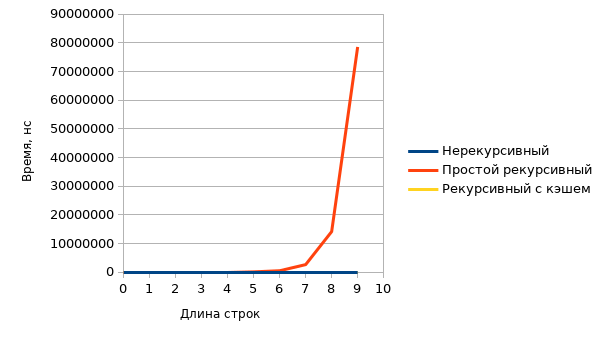
\includegraphics[width=\textwidth]{plt-01.png}
    \caption{Сравнение времени работы реализаций трёх алгоритмов}
\end{figure}

Поскольку простой рекурсивный алгоритм имеет, судя по результатам,
экспоненциальную временную сложность, были выполнены дополнительные
замеры процессорного времени выполнения реализаций двух оставшихся
алгоритмов.

\begin{figure}[ht]
    \centering
    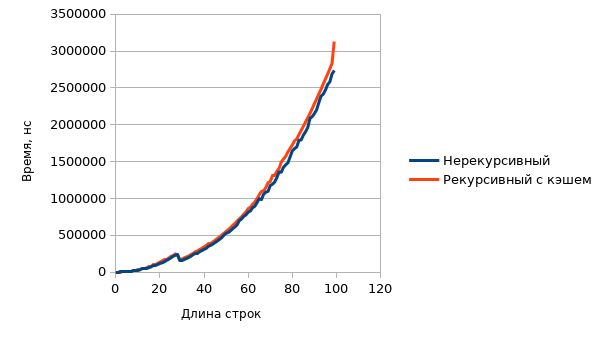
\includegraphics[width=\textwidth]{plt-02.png}
    \caption{Сравнение времени работы реализаций двух алгоритмов}
\end{figure}

\section{Оценка требуемой памяти}

В ходе работы был оценён объём требуемой для работы реализаций
памяти. Пусть одно беззнаковое целое число занимает $u$ памяти.

Нерекурсивный алгоритм в худшем случае требует:

\begin{itemize}
    \item $mn \cdot u$ памяти под матрицу;
    \item $2u$ памяти под счётчики $i$ и $j$;
    \item $4u$ памяти под случаи $a$, $b$, $c$ и $d$.
\end{itemize}

Итого: $(mn + 6)u$.

Простой рекурсивный алгоритм в худшем случае каждый вызов требует:

\begin{itemize}
    \item $4u$ памяти под случаи $a$, $b$, $c$ и $d$.
\end{itemize}

Стоит отметить, что число его вызовов растёт экспоненциально.
Итого: $4u \cdot a^{mn}$.

Рекурсивный алгоритм с кэшем требует:

\begin{itemize}
    \item $mn \cdot u$ памяти под кэш.
\end{itemize}

Кроме того, каждый вызов он требует:

\begin{itemize}
    \item $4u$ памяти под случаи $a$, $b$, $c$ и $d$.
\end{itemize}

Итого: $mn \cdot u + 4u \cdot b^{mn}$.

\section{Выводы}

Самым эффективным алгоритом поиска расстояния Дамерау-Левенштейна
как по времени, так и по памяти, оказался нерекурсивный алгоритм.

\chapter*{Заключение}
\addcontentsline{toc}{chapter}{Заключение}

В ходе работы были решены следующие задачи:

\begin{enumerate}
    \item изучены расстояния Левенштейна и Дамерау-Левенштейна;
    \item разработаны алгоритмы поиска изученных расстояний;
    \item реализованы разработанные алгоритмы;
    \item выполнены замеры процессорного времени работы реализаций;
    \item оценён объём требуемой для работы реализаций памяти;
    \item выполнен сравнительный анализ разработанных алгоритмов.
\end{enumerate}

Был изучен метод динамического программирования на примере
реализации алгоритмов поиска расстояний Левенштейна и
Дамерау-Левенштейна.

\chapter*{Список литературы}
\addcontentsline{toc}{chapter}{Список литературы}

1. Левенштейн, В. И. Двоичные коды с исправлением выпадений,
вставок и замещений символов. / В. И. Левенштейн // Доклады
Академий Наук СССР. -- 1965. -- 163.4. -- 845-848.

2. Damerau, F. J. A technique for computer detection and correction
of spelling errors. / F. J. Damerau // Communications of the ACM.
-- 1964. -- 7 (3). -- 171-176.

3. Colomiets, P. CPU Time Measurement Library. / P. Colomiets
URL: https://crates.io/crates/cpu-time
(дата обращения: 30.09.2022).

\end{document}
